\documentclass[12pt,a4paper,titlepage]{article}
\usepackage[utf8]{inputenc}
\usepackage{csquotes}
\usepackage[T1]{fontenc}
\usepackage{amsmath}
\usepackage{amsfonts}
\usepackage{amssymb}
\usepackage[left=3cm,right=3cm,top=2.5cm,bottom=2.5cm]{geometry}
\usepackage{url}
\usepackage[czech]{babel}
\usepackage[
  backend=biber,
  style=iso-numeric
]{biblatex}
\addbibresource{maturitni_prace.bib}
\usepackage{graphicx}
\usepackage[]{fancyvrb}
\usepackage[]{color}
\usepackage{url}
\graphicspath{ {./images/} }

\usepackage{setspace}
\fontfamily{ptm}
\usepackage{tabularx,ragged2e,booktabs}

\DeclareBibliographyCategory{skipbibliography}
\DeclareCiteCommand{\fcite}[\mkbibfootnote]
  {\usebibmacro{prenote}}
  {\addtocategory{skipbibliography}{\thefield{entrykey}}%
   \usedriver
     {\DeclareNameAlias{sortname}{default}}
     {\thefield{entrytype}}}
  {\multicitedelim}
  {\usebibmacro{postnote}}

\author{Antonín Vřešťál}
\title{Tvorba astronomických videí}
\renewcommand{\baselinestretch}{1.5} 


\begin{document}
\maketitle

\tableofcontents
\newpage
Prohlášení a poděkování přijde sem
\newpage
\part{Teoretická část}
\section{Postup vytváření videa}
\subsection{Výběr téma a shromažďování podkladů (WIP)}
Výběr témat začíná vždy konverzací mezi jednotlivými členy. Faktory které řešíme jsou aktuální události, možnost jednotlivých členů pracovat a nálada v celém kolektivu ohledně daného téma. Následně se společně dohodneme na věcech, které bychom rádi v případném videu na dané téma probrali. (zde i v další části přijde část s Danem [naším editorem] a Terkou [naší dabérkou], kterou ještě nemám)
\subsection{Příprava textových a zvukových podkladů}
\subsection{Animování oblohy v programu Stellárium} \label{makingof:stellarium}
Celý proces začíná se scénářem. Ze scénáře si vypíši seznam přechodů a jednotlivých scén. Pro tento úkol jsem si vytvořil speciální formát zápisu, který zachytává vše, co budu potřebovat k vytvoření každého přechodu ve videu. Viz tabulka \ref{tab:scenar}.
Většina animací, které se v těchto videích nachází, byly vytvořeny pomocí simulačního programu Stellarium. Tento program je open-source (jeho zdrojový kód je volně dostupný) a jeho oficiálním účelem je realistická simulace noční oblohy při pohledu očima nebo dalekohledem\fcite{stellarium:homepage}. Stellarium poskytuje širokou nabídku programovatelných rozhraní, ať už webový server, přes který lze instanci Stellaria ovládat z prohlížeče nebo skriptovací rozhraní, které umožňuje interakci s většinou částí Stellaria pomocí programovacího jazyka, založeného na standardu ECMAScript, využívaného například jazykem JavaScript nebo ActionScript\fcite{wiki:ecmascript}.

Největším problémem pro využití Stellaria v produkci videí je fakt, že Stellarium není pro tento úkol stavěno. Neexistuje žádná funkce, která by Stellariu řekla \enquote{Otoč se plynule na tyto souřadnice a při tom vytvoř video}. Jediná možnost tvorby videa je export každého snímku finálního jako separátní soubor a tyto jednotlivé soubory poté spojit pomocí nástroje jako FFmpeg. Zde ale vznikne další problém. Tyto jednotlivé snímky musí být rovnoměrně rozloženy po celé trajektorii přechodu. Tento problém je jeden z nejobvyklejších problémů a také důvod, proč jsem přešel od manuálních animací k plně automatizovaným skriptům. Tento problém se nejčastěji řeší pomocí lineární interpolace. Základní rovnici této transformace můžete vidět níže.
\[c = (1-t)*a + t * b\] 
Kde $t$ představuje faktor v intervalu $\langle0;1\rangle$, který postupně interpoluje mezi hodnotami $a$ a $b$. Tento přechod je těžko vizualizovatelný v papírové podobě a je tedy dostupný na \url{https://c.itoncek.space/maturitni_prace/lerp_1}

\textbf{Stará verze}

Celý proces začíná se scénářem. Ze scénáře si vypíši seznam přechodů a jednotlivých scén. Pro tento úkol jsem si vytvořil speciální formát zápisu, který zachytává vše, co budu potřebovat k vytvoření každého přechodu ve videu. Viz tabulka \ref{tab:scenar}. 
Pro kompozici těchto videí používám planetární program Stellarium. \textit{Stellarium je počítačový program pro simulaci planetária. [...] Využívá grafickou knihovnu OpenGL pro renderování téměř realistické třírozměrné oblohy v reálném čase.} \fcite{wiki:stellarium} Tento program využíváme hlavně díky jeho vysoké kvalitě simulace a dostupnosti detailní dokumentace celého prostředí. Pro interakci se Stelláriem nyní využíváme vestavěnou funkci skriptování. Celý proces využívá nestandardní využití Stellária. Obvykle se Stellárium využívá pro simulaci noční oblohy v reálném čase pro plánování pozorování. Skripty, které pro Stellárium vytvářím sestávají z opakovaných příkazů otočení, přiblížení a vyfocení snímku pomocí interních funkcí Stellária. Do nástroje, který jsem si pro tento účel naprogramoval, vložím čas, azimut, výšku a zvětšení prvního a posledního snímku. Následně tento nástroj rozdělí vstupní hodnoty pro začátek i konec na pětidimenzionální vektor, ve kterém se čas rozdělí na složku data a složku času v rámci jednoho dne. Následně pomocí rovnice $c = (1-x)*a + x * b$, kde $x \in \langle0;1\rangle$ a hodnota $a$ je počáteční hodnotou pro jednu dimenzi a hodnota $b$ je koncovou hodnotou pro danou dimenzi, vyjde $c$ jako hodnota v bodě $x$ daného přechodu. Tomuto procesu se říká lineární interpolace. Tato operace se využívá hojně v animacích jako můstek ke složitějším algoritmům. 

V základní lineární interpolaci se hodnota $x$ mění lineárně na intervalu $x \in \langle0;1\rangle$, což znamená že vzdálenost mezi body je pokaždé stejná a je rovna délce přechodu dělené počtem bodů minus 1. Při tvorbě videí ale má čistá lineární interpolace výrazné problémy. Začátek a konec přechodu je trhaný a celý přechod je tak trochu trhnutý. Proto využíváme lehce modifikovanou verzi lineární interpolace, kde $x$ nejdříve propustíme skrze následující rovnici $x_{smooth} = (1 - t) * t^2 + t * (1-(1-x)^2))$, která pro $x in \langle0;1\rangle$ provede kvadratickou interpolaci začátku i konce. Toto má za následek plynulejší začátek a konec a tím pádem i plynulejší zdání celého přechodu. Následně skript obsahuje několik příkazů pro vyfocení statických fotografií. Tyto fotografie jsou při střihu využity na spojení jednotlivých přechodů a vizuální demonstraci probíraného tématu. Pomocí této šablony poté vygeneruji skript s 500 snímky animace a dvěma až šesti statickými snímky, který poté spustím ve Stelláriu a nechám vygenerovat všechny snímky na disk.

Pro ukládání využívám formát TIFF, který mi poskytuje vysoce kvalitní data, která jsou komprimována pouze bezztrátově pomocí algoritmu LZW. Jeden takový snímek má rozlišení 3840 na 2160 pixelů a velikost mezi pěti až sedmi megabajty. Dohromady má jeden přechod na disku velikost přibližně 7GB. Pro celé video by toto znamenalo velikost přes 200GB, což nejsem schopen uložit na dostatečně rychlém disku pro střih. Proto v posledním kroku příprav převedu každý přechod do formátu ProRes, který mi umožňuje tuto velikost snížit na pouhých 10GB, i za cenu malé ztráty na kvalitě. Při kompilaci jednotlivých snímků do videí také nastavím finální snímkovací frekvenci projektu, jíž je pro AstroCrew 50 sn./s.
\subsection{Kompletace videa v programu DaVinci Resolve} \label{makingof:resolve}
\subsubsection{Spojování jednotlivých částí} \label{makingof:resolve:merging}
Poté co je nahrán zvuk a vytvořeny veškeré animace následuje finální kompletace všech složek do finálního videa. Zde se poprvé potkává hlasová a obrazová složka. Na začátku každého videa máme několik videí, zatím co uvádíme obsah videa. Tato videa jsou s vesmírnou tématikou a častým kandidátem jsou záběry z mezinárodní vesmírné stanice, jelikož podléhají minimálním autorským právům. Po úvodním slovu a upozornění ohledně pravdivosti informací ve videu v závislosti na pozici pozorovatele na zemi přijde hlavní část videa. Zde se začínají přes sebe překrývat soubory vytvořené v sekci \ref{makingof:stellarium}. 

První scéna začíná bez jakýchkoliv souhvězdích viditelných a postupně jak video pokračuje, objevují se postupně další souhvězdí. Následující scény se drží velice podobné struktury, která je vidět na obrázku \ref{img:timeline}. Na začátku, a ve speciálních případech i uprostřed scény, se vyskytují animace, které jsou na snímku označeny číslem 1. V průběhu scény je jako podklad využit statický snímek, vygenerovaný v sekci \ref{makingof:stellarium}. Tento snímek je označený číslem 2 a slouží jako základ každé scény, přes který jsou poté překryty snímky souhvěždí (3) a objektů hlubokého vesmíru (5). Pro větší názornost využíváme tzv. pointer (4), animovaný klip pulzijícího čtverce se zaoblenými rohy, jež zvýrazňuje část obrazu o kterém právě pojednává scénář, jehož vizuální reprezentace je vidět jako obrázek \ref{img:pointer} . Někdy je třeba zvýraznit zvolený objekt hlubokého vesmíru na úkor pozadí, které zrovna v daném momentě není důležité. V tomto snímku je tento tzv. Adjustment Clip vidět pod číslem 6. Zvuková část se po většinu času skládá ze dvou stop: hlasové stopy (7) a hudební stopy (8). Hlasová stopa se nachází primárně mimo animace, kdy její dominantní místo nahradí hudba, která je po dobu přechodů zesílena.

Nad scénou se nachází pět až šest stop s titulky. Tyto stopy využíváme nejen pro standardní využití ve formě titulků v Češtině a někdy i v Angličtině, ale využíváme je i jako prostor pro citování zdrojů obrazových materiálů, opravě chyb v již vydaném videu, poznámky a doplnění obsahu od editora a stopa s informacemi a zdrojích hudby. Tento postup využíváme hlavně kvůli jednoduchosti tvorby titulků a možnosti tyto titulky skrýt a nebýt jimi rušen. 

Souhvězdí a objekty hlubokého vesmíru jsou řazeny podle nejlepšího času pozorování od západu slunce k východu slunce. Poté nastává část, kde zmíníme nejdůležitější události, které v průběhu měsíce nastávají. Na tomto místě zmiňujeme meteorické roje a atmosférické i vesmírné úkazy, které se mohou v průběhu měsíce ukázat.
\subsubsection{Mixování obrazové části}
Záběry jsou vrstveny přes sebe pomocí metody Lighten. Tato metoda pro každý pixel vypočítá barvu podle rovnice $[\max(r_1, r_2), \max(g_1, g_2), \max(b_1, b_2)]$,\fcite{wiki:blend} kde tato množina představuje červený, zelený a modrý kanál v tomto pořadí. Toto umožňuje světlým obrázkům souhvězdí překrývat se, aniž by bylo třeba odstraňovat u každého pozadí. Tento způsob mixování také využívám pro fotografie objektů hlubokého vesmíru. 

Nejdříve získám obrázek daného objektu z internetu. Nejčastějším zdrojem je Wikipedie, která poskytuje jasné licenční podmínky. Pokud na Wikipedie nemá vhodný nebo dostatečně kvalitní obrázek, začnu hledat po internetu další fotografie. Občas ani tento krok nepomůže, zvláště u objektů nezajímavých pro focení. V tomto případě se otočím na celooblohové sady dat, například Digitized Sky Survey 2 nebo Mellinger color optical survey které získávám z Centra astronomických dat univerzity ve Štrasburku díky jejich nástroji Aladin. Tyto sady dat pokrývají značný zlomek celé oblohy a z geografické pozice České republiky pokrývají 100\% viditelné oblohy. Tyto fotografie následně upravuji pomocí software Zoner Photo Studio X, kde upravím kontrast pozadí tak, aby bylo absolutně černé a tudíž při kompletaci zmizelo. Následně odstraním hvězdy blízko okraje snímku, aby byl přechod mezi snímkem a pozadím méně znatelný. Tyto fotografie jsou následně překrývány přes souhvězdí a pozadí. 
\section{Mechanismy kontroly správnosti obsahu a formy (WIP)}
\section{Specifika tvorby obecného videa(WIP)}
\section{Historie a vývoj procesu tvorby astronomických videí (WIP)}
Proces tvorby našich astronomických videí se v průběhu let drasticky změnil. První video jsme vytvořili v roce 2021 a od té doby jich vzniklo dalších 10\footnote{Započítávám zatím nevydaná videa, která budou vydaná do data maturitních zkoušek}.V této části se podíváme na celou historii tvorby astronomických videí skupinou AstroCrew.
\subsection{Začátky - Prosinec 2021}
Naše cesta začala v prosinci roku 2021. Zde jsme 14. prosince vydali naše první video. Toto video nebylo primárně určené k vydání na platformě YouTube ale bylo připraveno pro planetárium v iQLandii, kde jsme ho představili již 9. prosince. Celé video je kvůli tomu promítnuto sféricky, jak můžete vidět na obrázku \ref{img:prosinec}. Pro YouTube jsme toto video modifikovali, aby ho YouTube vzal jako 360° video, i když polovina videa je čistě černá. Co se týče produkce, toto video bylo velice náročné. Stříhací program, kterým byl v té době ještě Adobe Premiere Pro, neustále padal, a obecně tvorba animací v té době probíhala ještě manuálně. Stellárium dává k dispozici webové rozhraní umožňující plnou kontrolu nad danou instancí Stellária. Toto video jsem natáčel tak, že jsem namířil Stellarium podobně, jako je namířená kopule planetária v iQLandii a poté jsem pomocí přesouvání času přemisťoval souhvězdí a jednotlivé objekty tak, aby byly co nejlépe vidět. Následně jsem pomocí programu Adobe After Effects vložil do scény obrázky daných objektů hlubokého vesmíru pomocí integrovaného efektu VR Converter. Díky technologii Adobe Dynamic Link jsem poté jen vložil kompozice z After Effects přímo do časové osy v Premiere Pro a nemusel jsem je exportovat. Bohužel tento přístup je neskutečně pomalý a drasticky snižuje výkonnost celého stříhacího programu. 
\newpage
\part{Praktická část}
\newpage
\part{Přílohy}
\begin{table}[h]
\centering
\begin{tabularx}{\linewidth}{lc*{5}{>{\RaggedRight\arraybackslash}X}}
\toprule
\# scény    & Směr scény & Čas          & Souhvězdí         & Speciální objekty      \\ \midrule
0000        & Z obzor    & západ slunce & Labuť, Lyra, Orel & Letní trojúhelník      \\ \addlinespace
0001        & SZ obzor   & západ slunce & dtto, Herkules    & Herkulův květináč, M13 \\ \addlinespace
0002        & Z obzor    & západ slunce & dtto              & -                      \\ \addlinespace
...         & ...        & ...          & ...               & ...                    \\ \bottomrule
\end{tabularx}
\caption{Demonstrace tabulky s informacemi o scénách}
\label{tab:scenar}
\end{table}
\begin{figure}[h]
\centering
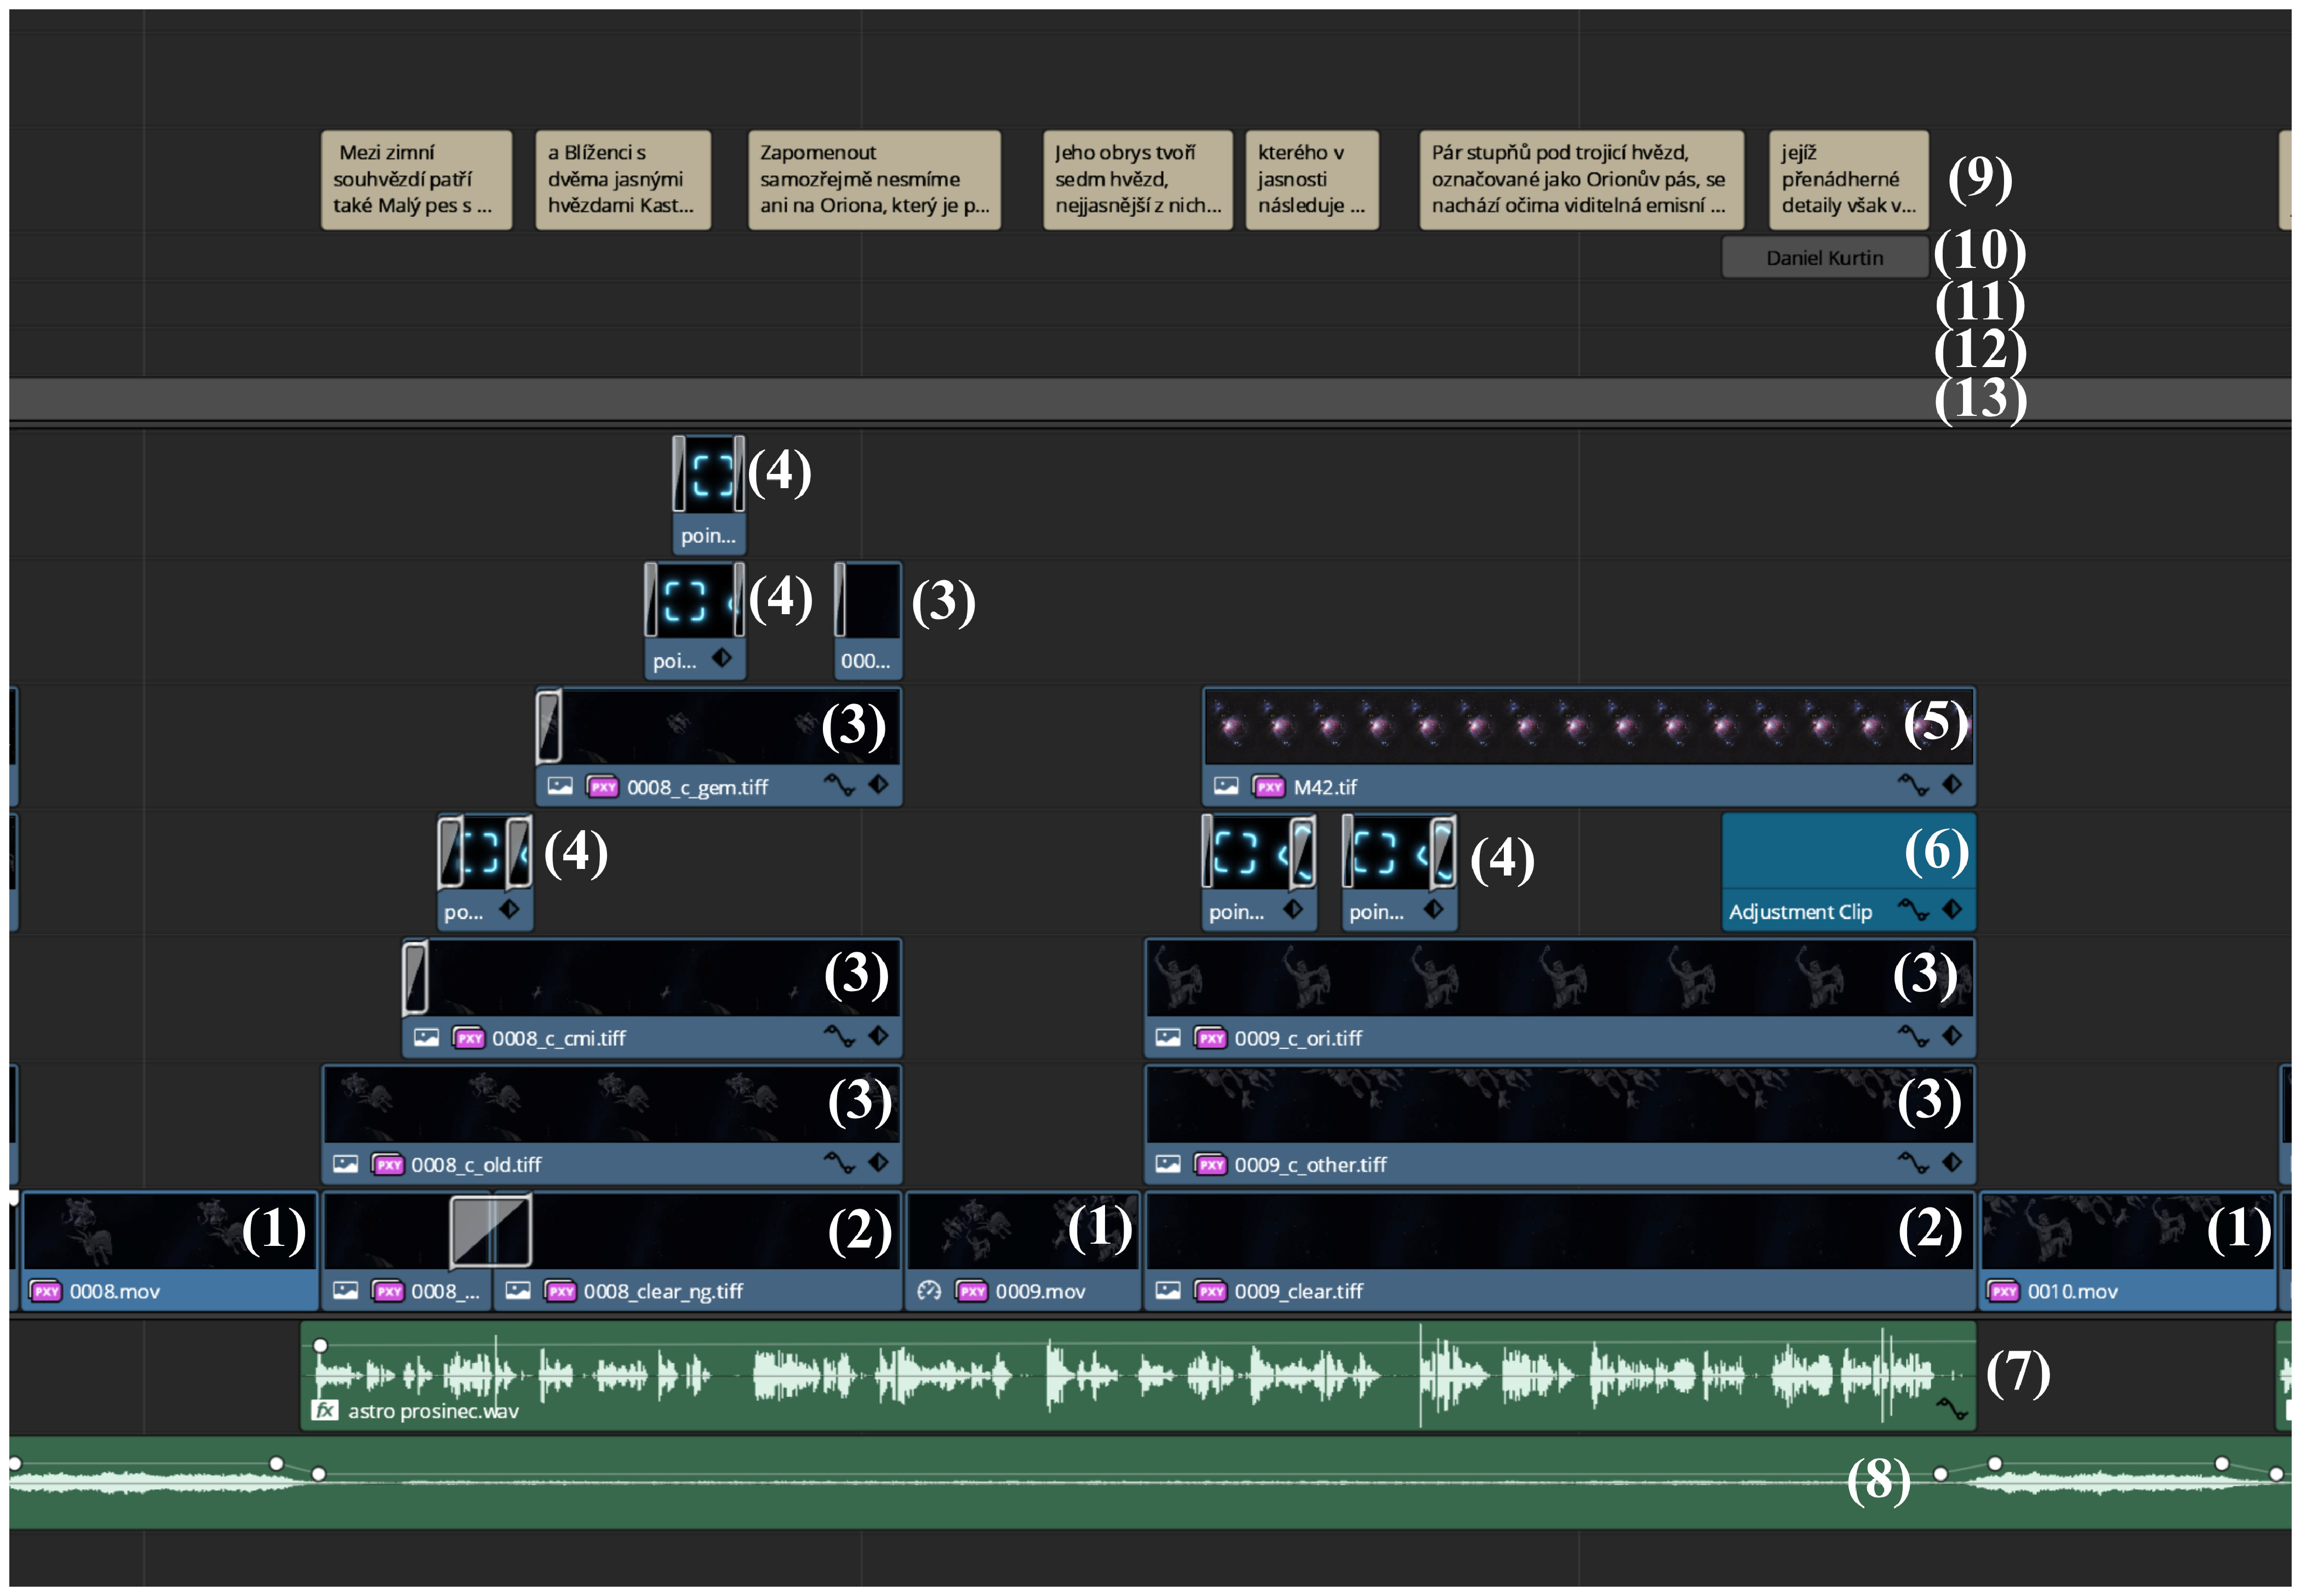
\includegraphics[width=1\textwidth]{timeline_annotated.eps}
\caption{Snímek jedné ze scén z finálního videa. Každá důležitá stopa má přiřazené číslo. Vysvětlení v oddílu \ref{makingof:resolve:merging}}
\label{img:timeline}
\end{figure}
\begin{figure}[ht]
\centering

\includegraphics[width=.5\textwidth]{pointer.eps}
\caption{Animace zvaná pointer, využívaná pro upřesnění pozice objektu, o kterém v daném momentě mluví scénář.}
\label{img:pointer}
\end{figure}
\begin{figure}[ht]
\centering
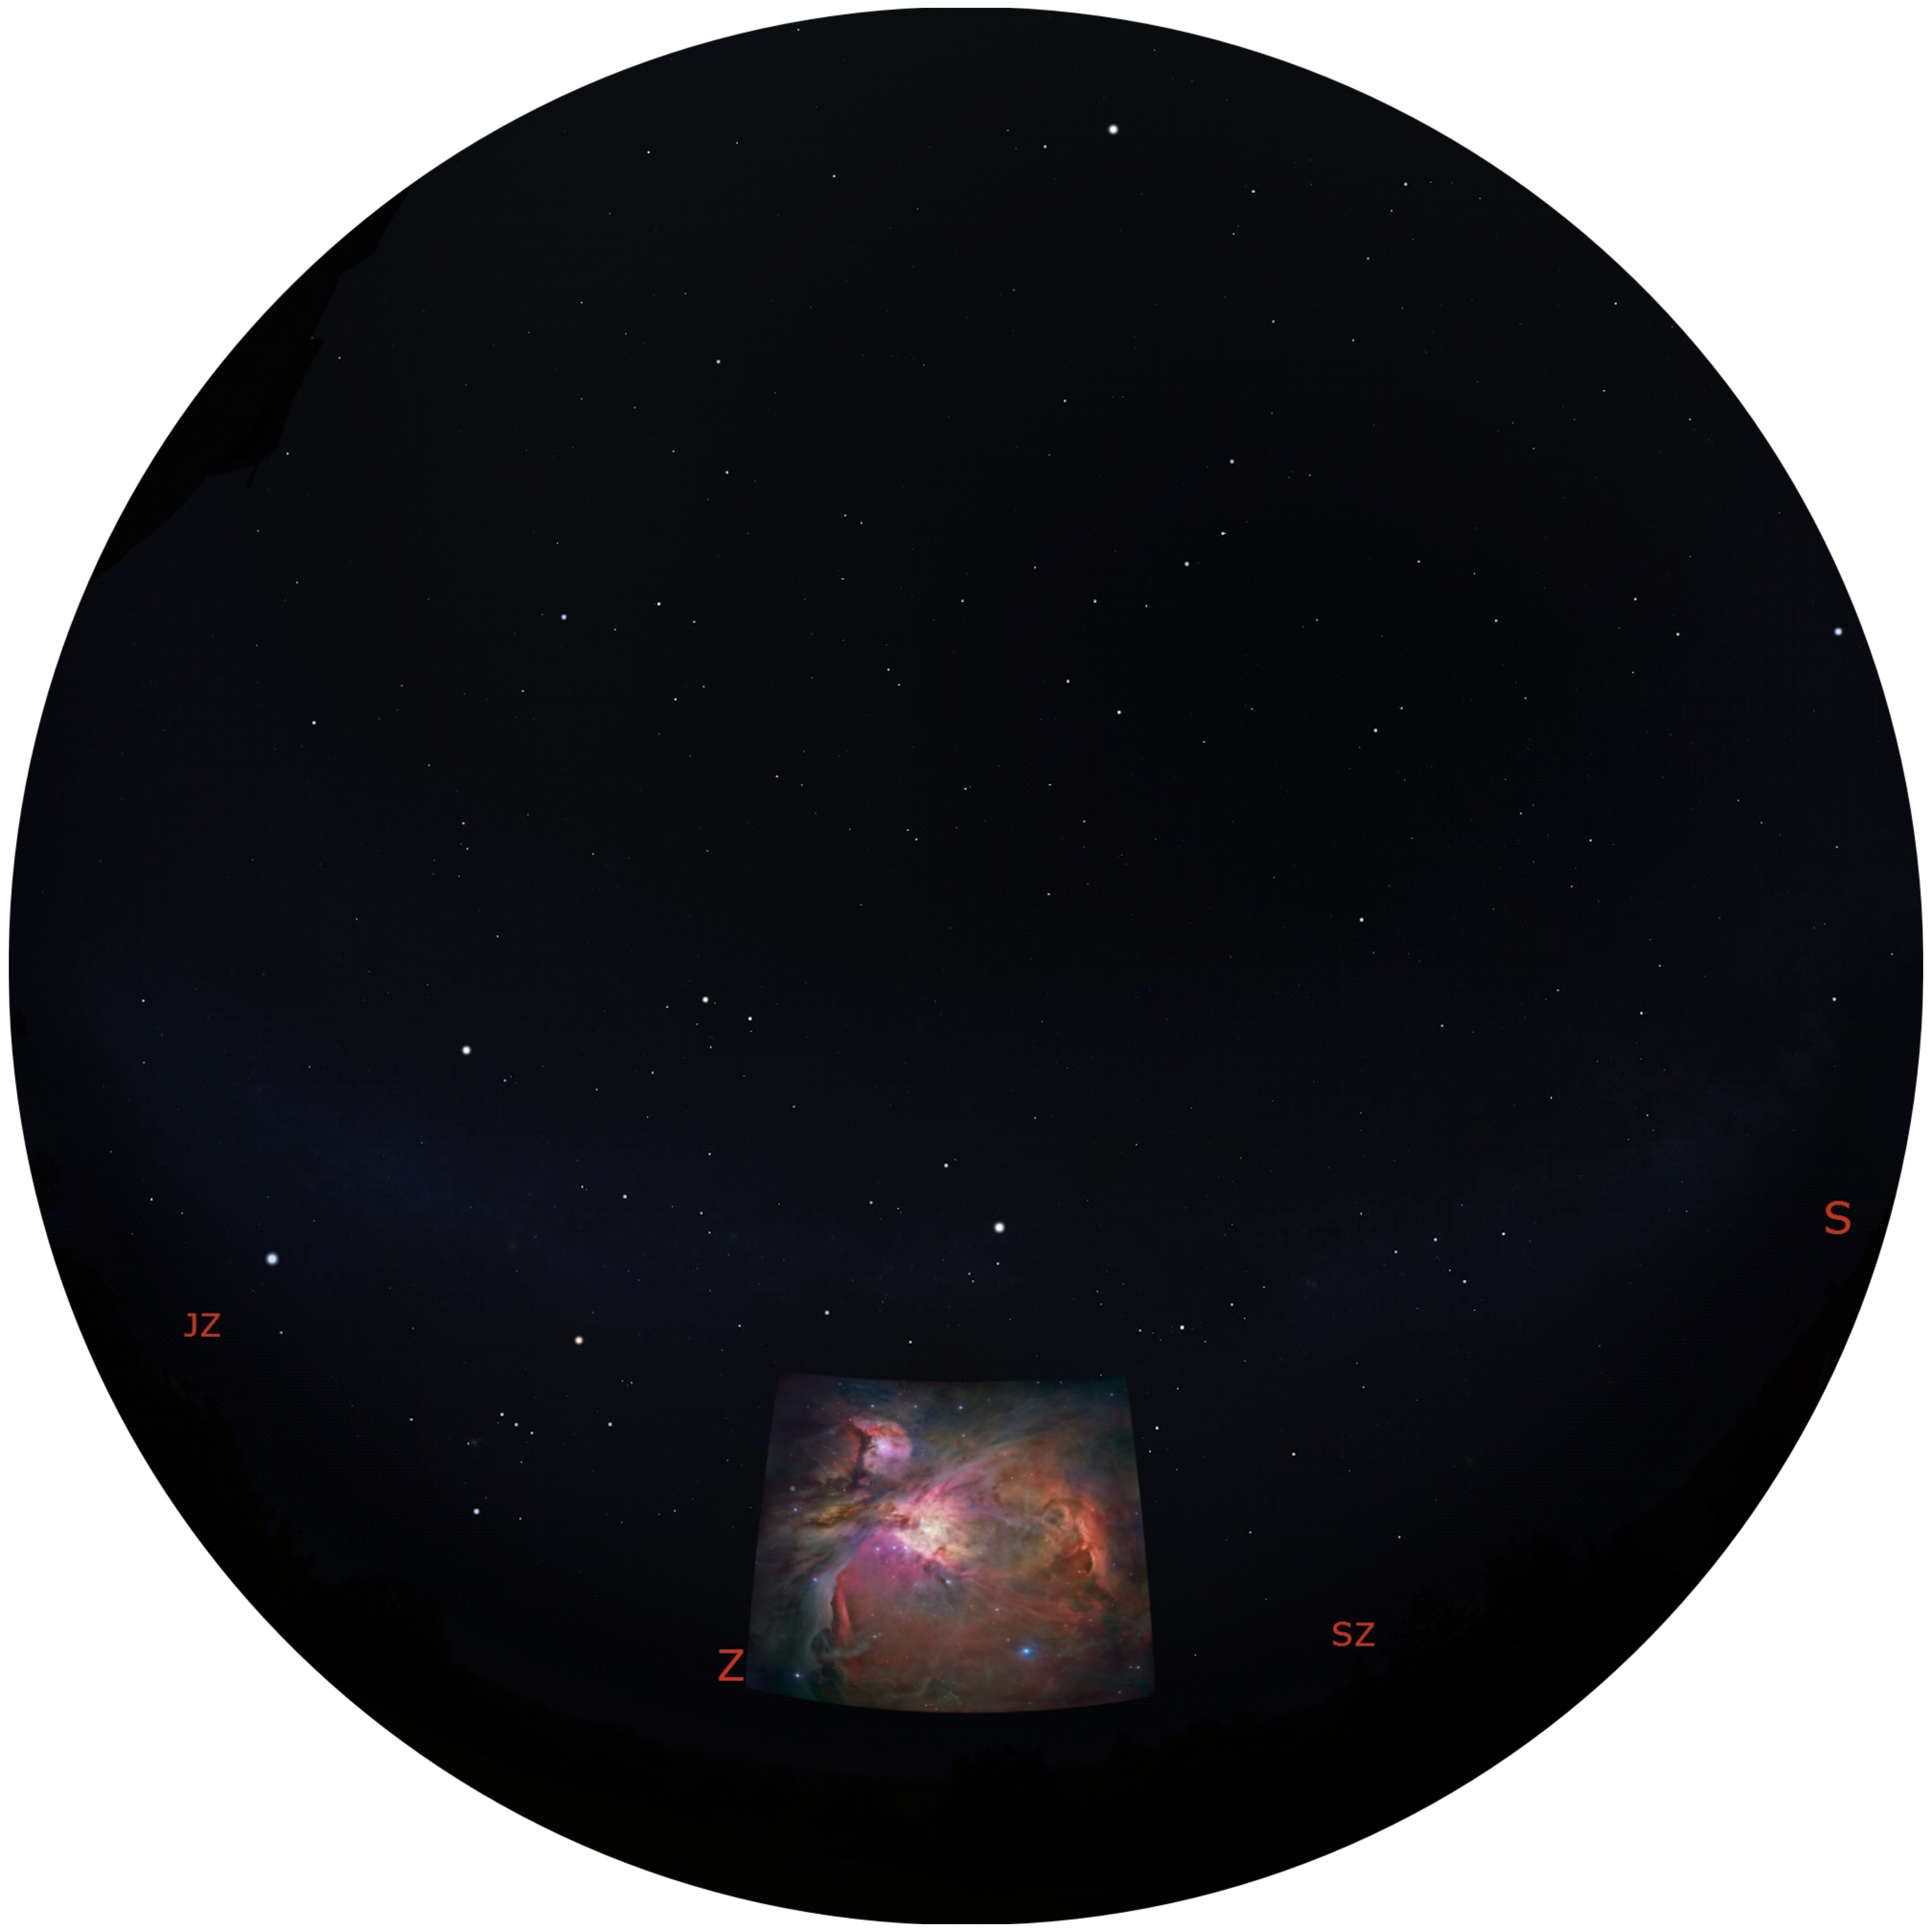
\includegraphics[width=.7\textwidth]{prosinec.eps}
\caption{Demonstrace našeho prvního videa.}
\label{img:prosinec}
\end{figure}

\end{document}